\begin{figure}[ht]
\begin{center}
\begin{adjustbox}{width=0.7\textwidth}

\tikzset{every picture/.style={line width=0.75pt}} %set default line width to 0.75pt        

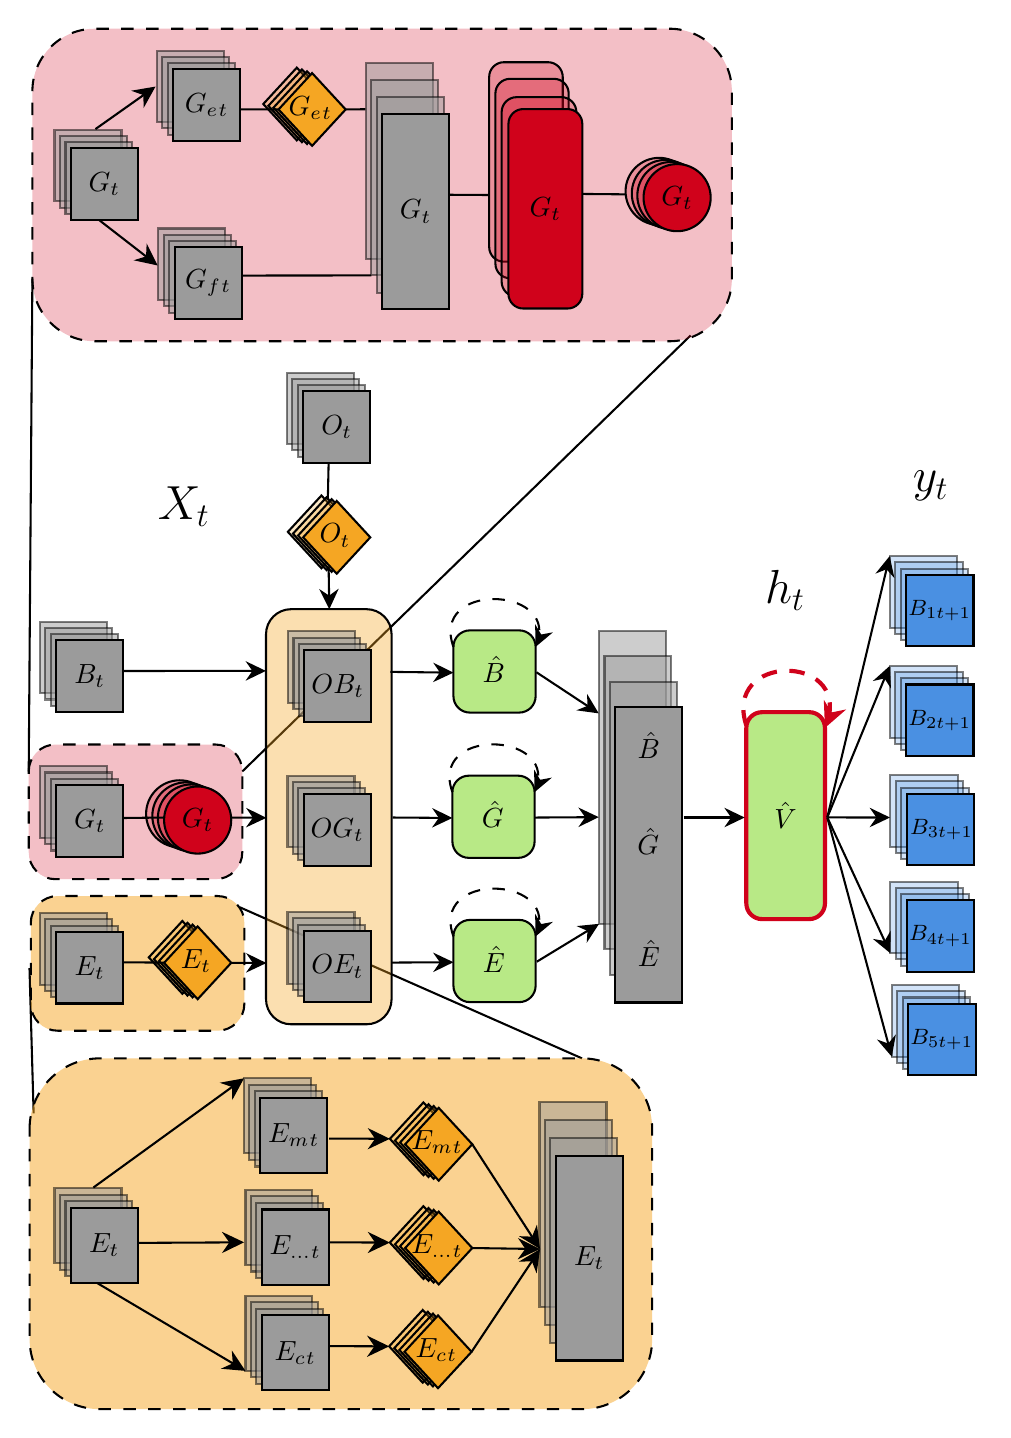
\begin{tikzpicture}[x=0.75pt,y=0.75pt,yscale=-1,xscale=1]
%uncomment if require: \path (0,846); %set diagram left start at 0, and has height of 846

%Straight Lines [id:da9103139984391558] 
\draw    (402.8,247.5) -- (186.8,457.57) ;
%Straight Lines [id:da3945923467366558] 
\draw    (84.27,552.33) -- (86.27,622.33) ;
%Straight Lines [id:da7710577267136013] 
\draw    (185.6,523) -- (350.47,595.8) ;
%Rounded Rect [id:dp8555004687770773] 
\draw  [fill={rgb, 255:red, 245; green, 166; blue, 35 }  ,fill opacity=0.5 ][dash pattern={on 4.5pt off 4.5pt}] (84.9,530.57) .. controls (84.9,523.4) and (90.71,517.59) .. (97.88,517.59) -- (174.83,517.59) .. controls (181.99,517.59) and (187.8,523.4) .. (187.8,530.57) -- (187.8,569.5) .. controls (187.8,576.67) and (181.99,582.48) .. (174.83,582.48) -- (97.88,582.48) .. controls (90.71,582.48) and (84.9,576.67) .. (84.9,569.5) -- cycle ;
%Rounded Rect [id:dp09236181577504154] 
\draw  [fill={rgb, 255:red, 208; green, 2; blue, 27 }  ,fill opacity=0.25 ][dash pattern={on 4.5pt off 4.5pt}] (83.9,457.57) .. controls (83.9,450.4) and (89.71,444.59) .. (96.88,444.59) -- (173.83,444.59) .. controls (180.99,444.59) and (186.8,450.4) .. (186.8,457.57) -- (186.8,496.5) .. controls (186.8,503.67) and (180.99,509.48) .. (173.83,509.48) -- (96.88,509.48) .. controls (89.71,509.48) and (83.9,503.67) .. (83.9,496.5) -- cycle ;
%Shape: Circle [id:dp7319115465111494] 
\draw  [fill={rgb, 255:red, 208; green, 2; blue, 27 }  ,fill opacity=0.25 ] (140.46,477.99) .. controls (140.46,469.06) and (147.7,461.82) .. (156.63,461.82) .. controls (165.56,461.82) and (172.8,469.06) .. (172.8,477.99) .. controls (172.8,486.91) and (165.56,494.15) .. (156.63,494.15) .. controls (147.7,494.15) and (140.46,486.91) .. (140.46,477.99) -- cycle ;
%Shape: Circle [id:dp20640118029319288] 
\draw  [fill={rgb, 255:red, 208; green, 2; blue, 27 }  ,fill opacity=0.25 ] (143.46,478.99) .. controls (143.46,470.06) and (150.7,462.82) .. (159.63,462.82) .. controls (168.56,462.82) and (175.8,470.06) .. (175.8,478.99) .. controls (175.8,487.91) and (168.56,495.15) .. (159.63,495.15) .. controls (150.7,495.15) and (143.46,487.91) .. (143.46,478.99) -- cycle ;
%Shape: Circle [id:dp9035374173552181] 
\draw  [fill={rgb, 255:red, 208; green, 2; blue, 27 }  ,fill opacity=0.25 ] (146.13,479.99) .. controls (146.13,471.06) and (153.37,463.82) .. (162.3,463.82) .. controls (171.23,463.82) and (178.47,471.06) .. (178.47,479.99) .. controls (178.47,488.91) and (171.23,496.15) .. (162.3,496.15) .. controls (153.37,496.15) and (146.13,488.91) .. (146.13,479.99) -- cycle ;
%Shape: Circle [id:dp2977025290564278] 
\draw  [fill={rgb, 255:red, 208; green, 2; blue, 27 }  ,fill opacity=1 ] (149.13,480.99) .. controls (149.13,472.06) and (156.37,464.82) .. (165.3,464.82) .. controls (174.23,464.82) and (181.47,472.06) .. (181.47,480.99) .. controls (181.47,489.91) and (174.23,497.15) .. (165.3,497.15) .. controls (156.37,497.15) and (149.13,489.91) .. (149.13,480.99) -- cycle ;

%Rounded Rect [id:dp11328404188335206] 
\draw  [fill={rgb, 255:red, 245; green, 166; blue, 35 }  ,fill opacity=0.36 ] (198.23,391.48) .. controls (198.23,384.8) and (203.65,379.38) .. (210.33,379.38) -- (246.63,379.38) .. controls (253.32,379.38) and (258.73,384.8) .. (258.73,391.48) -- (258.73,567.28) .. controls (258.73,573.97) and (253.32,579.38) .. (246.63,579.38) -- (210.33,579.38) .. controls (203.65,579.38) and (198.23,573.97) .. (198.23,567.28) -- cycle ;
%Straight Lines [id:da97742141306228] 
\draw    (228.39,359.09) -- (228.68,376.38) ;
\draw [shift={(228.73,379.38)}, rotate = 269.03] [fill={rgb, 255:red, 0; green, 0; blue, 0 }  ][line width=0.08]  [draw opacity=0] (9.82,-4.72) -- (0,0) -- (9.82,4.72) -- (6.52,0) -- cycle    ;
%Shape: Rectangle [id:dp41315418456735886] 
\draw  [color={rgb, 255:red, 0; green, 0; blue, 0 }  ,draw opacity=0.5 ][fill={rgb, 255:red, 155; green, 155; blue, 155 }  ,fill opacity=0.5 ] (89.34,525.86) -- (121.6,525.86) -- (121.6,560.38) -- (89.34,560.38) -- cycle ;
%Shape: Rectangle [id:dp3325769721726205] 
\draw  [color={rgb, 255:red, 0; green, 0; blue, 0 }  ,draw opacity=0.5 ][fill={rgb, 255:red, 155; green, 155; blue, 155 }  ,fill opacity=0.5 ] (91.96,528.84) -- (124.22,528.84) -- (124.22,563.36) -- (91.96,563.36) -- cycle ;
%Shape: Rectangle [id:dp41249766049421643] 
\draw  [color={rgb, 255:red, 0; green, 0; blue, 0 }  ,draw opacity=0.5 ][fill={rgb, 255:red, 155; green, 155; blue, 155 }  ,fill opacity=0.5 ] (94.61,531.9) -- (126.86,531.9) -- (126.86,566.41) -- (94.61,566.41) -- cycle ;
%Shape: Rectangle [id:dp7785272856806607] 
\draw  [fill={rgb, 255:red, 155; green, 155; blue, 155 }  ,fill opacity=1 ] (97.19,534.83) -- (129.45,534.83) -- (129.45,569.35) -- (97.19,569.35) -- cycle ;
%Straight Lines [id:da7676416072071721] 
\draw    (228.39,309.19) -- (228.01,326.76) ;
%Rounded Rect [id:dp3241527411138243] 
\draw  [color={rgb, 255:red, 208; green, 2; blue, 27 }  ,draw opacity=1 ][fill={rgb, 255:red, 184; green, 233; blue, 134 }  ,fill opacity=1 ][line width=1.5]  (429.64,436.58) .. controls (429.64,432.4) and (433.03,429) .. (437.22,429) -- (459.95,429) .. controls (464.14,429) and (467.53,432.4) .. (467.53,436.58) -- (467.53,521.12) .. controls (467.53,525.31) and (464.14,528.7) .. (459.95,528.7) -- (437.22,528.7) .. controls (433.03,528.7) and (429.64,525.31) .. (429.64,521.12) -- cycle ;
%Curve Lines [id:da04419993566075786] 
\draw [color={rgb, 255:red, 208; green, 2; blue, 27 }  ,draw opacity=1 ][line width=1.5]  [dash pattern={on 5.63pt off 4.5pt}]  (429.64,435.36) .. controls (418.28,400.73) and (478.54,400.66) .. (468.87,432.94) ;
\draw [shift={(467.53,436.58)}, rotate = 293.32] [fill={rgb, 255:red, 208; green, 2; blue, 27 }  ,fill opacity=1 ][line width=0.08]  [draw opacity=0] (12.23,-5.88) -- (0,0) -- (12.23,5.88) -- (8.12,0) -- cycle    ;
%Shape: Rectangle [id:dp4565115121522617] 
\draw  [color={rgb, 255:red, 0; green, 0; blue, 0 }  ,draw opacity=0.5 ][fill={rgb, 255:red, 74; green, 144; blue, 226 }  ,fill opacity=0.25 ] (498.7,406.73) -- (531.2,406.73) -- (531.2,441.23) -- (498.7,441.23) -- cycle ;
%Shape: Rectangle [id:dp4609539681268845] 
\draw  [color={rgb, 255:red, 0; green, 0; blue, 0 }  ,draw opacity=0.5 ][fill={rgb, 255:red, 74; green, 144; blue, 226 }  ,fill opacity=0.25 ] (501.34,409.7) -- (533.84,409.7) -- (533.84,444.21) -- (501.34,444.21) -- cycle ;
%Shape: Rectangle [id:dp8789374722188051] 
\draw  [color={rgb, 255:red, 0; green, 0; blue, 0 }  ,draw opacity=0.5 ][fill={rgb, 255:red, 74; green, 144; blue, 226 }  ,fill opacity=0.25 ] (504,412.76) -- (536.51,412.76) -- (536.51,447.26) -- (504,447.26) -- cycle ;
%Shape: Rectangle [id:dp5155508462057329] 
\draw  [fill={rgb, 255:red, 74; green, 144; blue, 226 }  ,fill opacity=1 ] (506.61,415.69) -- (539.11,415.69) -- (539.11,450.2) -- (506.61,450.2) -- cycle ;
%Shape: Rectangle [id:dp7477154343750577] 
\draw  [color={rgb, 255:red, 0; green, 0; blue, 0 }  ,draw opacity=0.5 ][fill={rgb, 255:red, 74; green, 144; blue, 226 }  ,fill opacity=0.25 ] (499.03,459.39) -- (531.53,459.39) -- (531.53,493.9) -- (499.03,493.9) -- cycle ;
%Shape: Rectangle [id:dp2965318097655928] 
\draw  [color={rgb, 255:red, 0; green, 0; blue, 0 }  ,draw opacity=0.5 ][fill={rgb, 255:red, 74; green, 144; blue, 226 }  ,fill opacity=0.25 ] (501.67,462.37) -- (534.17,462.37) -- (534.17,496.88) -- (501.67,496.88) -- cycle ;
%Shape: Rectangle [id:dp2218344689056715] 
\draw  [color={rgb, 255:red, 0; green, 0; blue, 0 }  ,draw opacity=0.5 ][fill={rgb, 255:red, 74; green, 144; blue, 226 }  ,fill opacity=0.25 ] (504.33,465.42) -- (536.84,465.42) -- (536.84,499.93) -- (504.33,499.93) -- cycle ;
%Shape: Rectangle [id:dp2989576386252515] 
\draw  [fill={rgb, 255:red, 74; green, 144; blue, 226 }  ,fill opacity=1 ] (506.95,468.36) -- (539.17,468.36) -- (539.17,502.56) -- (506.95,502.56) -- cycle ;
%Shape: Rectangle [id:dp8259746733237621] 
\draw  [color={rgb, 255:red, 0; green, 0; blue, 0 }  ,draw opacity=0.5 ][fill={rgb, 255:red, 74; green, 144; blue, 226 }  ,fill opacity=0.25 ] (499.7,560.45) -- (532.2,560.45) -- (532.2,594.95) -- (499.7,594.95) -- cycle ;
%Shape: Rectangle [id:dp9996763094067804] 
\draw  [color={rgb, 255:red, 0; green, 0; blue, 0 }  ,draw opacity=0.5 ][fill={rgb, 255:red, 74; green, 144; blue, 226 }  ,fill opacity=0.25 ] (502.34,563.42) -- (534.84,563.42) -- (534.84,597.93) -- (502.34,597.93) -- cycle ;
%Shape: Rectangle [id:dp4217803468736018] 
\draw  [color={rgb, 255:red, 0; green, 0; blue, 0 }  ,draw opacity=0.5 ][fill={rgb, 255:red, 74; green, 144; blue, 226 }  ,fill opacity=0.25 ] (505,566.48) -- (537.51,566.48) -- (537.51,600.98) -- (505,600.98) -- cycle ;
%Shape: Rectangle [id:dp09858187105260652] 
\draw  [fill={rgb, 255:red, 74; green, 144; blue, 226 }  ,fill opacity=1 ] (507.61,569.41) -- (540.11,569.41) -- (540.11,603.92) -- (507.61,603.92) -- cycle ;

%Shape: Rectangle [id:dp8496590185951295] 
\draw  [color={rgb, 255:red, 0; green, 0; blue, 0 }  ,draw opacity=0.5 ][fill={rgb, 255:red, 74; green, 144; blue, 226 }  ,fill opacity=0.25 ] (499.03,510.66) -- (531.53,510.66) -- (531.53,545.16) -- (499.03,545.16) -- cycle ;
%Shape: Rectangle [id:dp5967326633998711] 
\draw  [color={rgb, 255:red, 0; green, 0; blue, 0 }  ,draw opacity=0.5 ][fill={rgb, 255:red, 74; green, 144; blue, 226 }  ,fill opacity=0.25 ] (501.67,513.63) -- (534.17,513.63) -- (534.17,548.14) -- (501.67,548.14) -- cycle ;
%Shape: Rectangle [id:dp4318566887941836] 
\draw  [color={rgb, 255:red, 0; green, 0; blue, 0 }  ,draw opacity=0.5 ][fill={rgb, 255:red, 74; green, 144; blue, 226 }  ,fill opacity=0.25 ] (504.33,516.69) -- (536.84,516.69) -- (536.84,551.19) -- (504.33,551.19) -- cycle ;
%Shape: Rectangle [id:dp19219507917553602] 
\draw  [fill={rgb, 255:red, 74; green, 144; blue, 226 }  ,fill opacity=1 ] (506.94,519.62) -- (539.44,519.62) -- (539.44,554.13) -- (506.94,554.13) -- cycle ;
%Shape: Rectangle [id:dp3520287753010958] 
\draw  [color={rgb, 255:red, 0; green, 0; blue, 0 }  ,draw opacity=0.5 ][fill={rgb, 255:red, 74; green, 144; blue, 226 }  ,fill opacity=0.25 ] (498.7,353.81) -- (531.2,353.81) -- (531.2,388.32) -- (498.7,388.32) -- cycle ;
%Shape: Rectangle [id:dp9540520643609552] 
\draw  [color={rgb, 255:red, 0; green, 0; blue, 0 }  ,draw opacity=0.5 ][fill={rgb, 255:red, 74; green, 144; blue, 226 }  ,fill opacity=0.25 ] (501.34,356.79) -- (533.84,356.79) -- (533.84,391.3) -- (501.34,391.3) -- cycle ;
%Shape: Rectangle [id:dp009162639846162945] 
\draw  [color={rgb, 255:red, 0; green, 0; blue, 0 }  ,draw opacity=0.5 ][fill={rgb, 255:red, 74; green, 144; blue, 226 }  ,fill opacity=0.25 ] (504,359.84) -- (536.51,359.84) -- (536.51,394.35) -- (504,394.35) -- cycle ;
%Shape: Rectangle [id:dp2786840324586616] 
\draw  [fill={rgb, 255:red, 74; green, 144; blue, 226 }  ,fill opacity=1 ] (506.61,362.78) -- (539.11,362.78) -- (539.11,397.28) -- (506.61,397.28) -- cycle ;
%Shape: Rectangle [id:dp9407625013058583] 
\draw  [color={rgb, 255:red, 0; green, 0; blue, 0 }  ,draw opacity=0.5 ][fill={rgb, 255:red, 155; green, 155; blue, 155 }  ,fill opacity=0.5 ] (89.34,455.11) -- (121.6,455.11) -- (121.6,489.62) -- (89.34,489.62) -- cycle ;
%Shape: Rectangle [id:dp8058750429381125] 
\draw  [color={rgb, 255:red, 0; green, 0; blue, 0 }  ,draw opacity=0.5 ][fill={rgb, 255:red, 155; green, 155; blue, 155 }  ,fill opacity=0.5 ] (91.96,458.08) -- (124.22,458.08) -- (124.22,492.6) -- (91.96,492.6) -- cycle ;
%Shape: Rectangle [id:dp5323246767908464] 
\draw  [color={rgb, 255:red, 0; green, 0; blue, 0 }  ,draw opacity=0.5 ][fill={rgb, 255:red, 155; green, 155; blue, 155 }  ,fill opacity=0.5 ] (94.61,461.14) -- (126.86,461.14) -- (126.86,495.65) -- (94.61,495.65) -- cycle ;
%Shape: Rectangle [id:dp89646361103016] 
\draw  [fill={rgb, 255:red, 155; green, 155; blue, 155 }  ,fill opacity=1 ] (97.19,464.07) -- (129.45,464.07) -- (129.45,498.59) -- (97.19,498.59) -- cycle ;
%Straight Lines [id:da3920605649543164] 
\draw [fill={rgb, 255:red, 155; green, 155; blue, 155 }  ,fill opacity=1 ]   (128.43,409.16) -- (195.19,409.13) ;
\draw [shift={(198.19,409.13)}, rotate = 179.98] [fill={rgb, 255:red, 0; green, 0; blue, 0 }  ][line width=0.08]  [draw opacity=0] (9.82,-4.72) -- (0,0) -- (9.82,4.72) -- (6.52,0) -- cycle    ;
%Shape: Rectangle [id:dp6850648570443139] 
\draw  [color={rgb, 255:red, 0; green, 0; blue, 0 }  ,draw opacity=0.5 ][fill={rgb, 255:red, 155; green, 155; blue, 155 }  ,fill opacity=0.5 ] (89.34,385.39) -- (121.6,385.39) -- (121.6,419.91) -- (89.34,419.91) -- cycle ;
%Shape: Rectangle [id:dp41277289741969747] 
\draw  [color={rgb, 255:red, 0; green, 0; blue, 0 }  ,draw opacity=0.5 ][fill={rgb, 255:red, 155; green, 155; blue, 155 }  ,fill opacity=0.5 ] (91.96,388.37) -- (124.22,388.37) -- (124.22,422.89) -- (91.96,422.89) -- cycle ;
%Shape: Rectangle [id:dp24642131513929277] 
\draw  [color={rgb, 255:red, 0; green, 0; blue, 0 }  ,draw opacity=0.5 ][fill={rgb, 255:red, 155; green, 155; blue, 155 }  ,fill opacity=0.5 ] (94.61,391.42) -- (126.86,391.42) -- (126.86,425.94) -- (94.61,425.94) -- cycle ;
%Shape: Rectangle [id:dp804695585404719] 
\draw  [fill={rgb, 255:red, 155; green, 155; blue, 155 }  ,fill opacity=1 ] (97.19,394.36) -- (129.45,394.36) -- (129.45,428.88) -- (97.19,428.88) -- cycle ;
%Straight Lines [id:da12400868298701306] 
\draw    (129.79,479.99) -- (149.13,479.77) ;
%Shape: Diamond [id:dp24460501554955205] 
\draw  [fill={rgb, 255:red, 245; green, 166; blue, 35 }  ,fill opacity=0.25 ] (157.93,529.62) -- (174.1,547.14) -- (157.93,564.66) -- (141.76,547.14) -- cycle ;
%Shape: Diamond [id:dp38612507244945715] 
\draw  [fill={rgb, 255:red, 245; green, 166; blue, 35 }  ,fill opacity=0.25 ] (160.39,530.49) -- (176.56,548.02) -- (160.39,565.54) -- (144.22,548.02) -- cycle ;
%Shape: Diamond [id:dp7294425738188043] 
\draw  [fill={rgb, 255:red, 245; green, 166; blue, 35 }  ,fill opacity=0.25 ] (162.84,531.37) -- (179.01,548.89) -- (162.84,566.41) -- (146.68,548.89) -- cycle ;
%Shape: Diamond [id:dp4600936139066173] 
\draw  [fill={rgb, 255:red, 245; green, 166; blue, 35 }  ,fill opacity=1 ] (165.3,532.25) -- (181.47,549.77) -- (165.3,567.29) -- (149.13,549.77) -- cycle ;
%Straight Lines [id:da04018115748321993] 
\draw    (181.47,549.77) -- (195.41,549.84) ;
\draw [shift={(198.41,549.86)}, rotate = 180.32] [fill={rgb, 255:red, 0; green, 0; blue, 0 }  ][line width=0.08]  [draw opacity=0] (9.82,-4.72) -- (0,0) -- (9.82,4.72) -- (6.52,0) -- cycle    ;
%Straight Lines [id:da67208321133131] 
\draw    (129.22,549.53) -- (149.22,549.65) ;
%Straight Lines [id:da48258650691324334] 
\draw [fill={rgb, 255:red, 155; green, 155; blue, 155 }  ,fill opacity=1 ]   (258.1,409.59) -- (285.53,409.93) ;
\draw [shift={(288.53,409.97)}, rotate = 180.71] [fill={rgb, 255:red, 0; green, 0; blue, 0 }  ][line width=0.08]  [draw opacity=0] (9.82,-4.72) -- (0,0) -- (9.82,4.72) -- (6.52,0) -- cycle    ;
%Rounded Rect [id:dp42275452319378204] 
\draw  [color={rgb, 255:red, 0; green, 0; blue, 0 }  ,draw opacity=1 ][fill={rgb, 255:red, 184; green, 233; blue, 134 }  ,fill opacity=1 ][line width=0.75]  (288.53,397.52) .. controls (288.53,393.15) and (292.08,389.6) .. (296.45,389.6) -- (320.21,389.6) .. controls (324.59,389.6) and (328.13,393.15) .. (328.13,397.52) -- (328.13,421.28) .. controls (328.13,425.65) and (324.59,429.2) .. (320.21,429.2) -- (296.45,429.2) .. controls (292.08,429.2) and (288.53,425.65) .. (288.53,421.28) -- cycle ;
%Curve Lines [id:da9780504206425155] 
\draw [color={rgb, 255:red, 0; green, 0; blue, 0 }  ,draw opacity=1 ][line width=0.75]  [dash pattern={on 4.5pt off 4.5pt}]  (288.53,397.52) .. controls (277.25,366.4) and (337.58,368.14) .. (329.12,394.96) ;
\draw [shift={(328.13,397.52)}, rotate = 294.37] [fill={rgb, 255:red, 0; green, 0; blue, 0 }  ,fill opacity=1 ][line width=0.08]  [draw opacity=0] (9.82,-4.72) -- (0,0) -- (9.82,4.72) -- (6.52,0) -- cycle    ;
%Straight Lines [id:da5158835638604321] 
\draw [fill={rgb, 255:red, 155; green, 155; blue, 155 }  ,fill opacity=1 ]   (328.53,409.78) -- (356.03,427.93) ;
\draw [shift={(358.53,429.58)}, rotate = 213.42] [fill={rgb, 255:red, 0; green, 0; blue, 0 }  ][line width=0.08]  [draw opacity=0] (9.82,-4.72) -- (0,0) -- (9.82,4.72) -- (6.52,0) -- cycle    ;
%Straight Lines [id:da9882019713778407] 
\draw    (181.47,479.77) -- (195.41,479.87) ;
\draw [shift={(198.41,479.9)}, rotate = 180.44] [fill={rgb, 255:red, 0; green, 0; blue, 0 }  ][line width=0.08]  [draw opacity=0] (9.82,-4.72) -- (0,0) -- (9.82,4.72) -- (6.52,0) -- cycle    ;
%Straight Lines [id:da48797669686945266] 
\draw [fill={rgb, 255:red, 155; green, 155; blue, 155 }  ,fill opacity=1 ]   (259.25,479.76) -- (285.03,479.95) ;
\draw [shift={(288.03,479.97)}, rotate = 180.41] [fill={rgb, 255:red, 0; green, 0; blue, 0 }  ][line width=0.08]  [draw opacity=0] (9.82,-4.72) -- (0,0) -- (9.82,4.72) -- (6.52,0) -- cycle    ;
%Rounded Rect [id:dp5436174431185763] 
\draw  [color={rgb, 255:red, 0; green, 0; blue, 0 }  ,draw opacity=1 ][fill={rgb, 255:red, 184; green, 233; blue, 134 }  ,fill opacity=1 ][line width=0.75]  (288.03,467.52) .. controls (288.03,463.15) and (291.58,459.6) .. (295.95,459.6) -- (319.71,459.6) .. controls (324.09,459.6) and (327.63,463.15) .. (327.63,467.52) -- (327.63,491.28) .. controls (327.63,495.65) and (324.09,499.2) .. (319.71,499.2) -- (295.95,499.2) .. controls (291.58,499.2) and (288.03,495.65) .. (288.03,491.28) -- cycle ;
%Curve Lines [id:da21188722634129087] 
\draw [color={rgb, 255:red, 0; green, 0; blue, 0 }  ,draw opacity=1 ][line width=0.75]  [dash pattern={on 4.5pt off 4.5pt}]  (288.03,467.52) .. controls (276.75,436.4) and (337.08,438.14) .. (328.62,464.96) ;
\draw [shift={(327.63,467.52)}, rotate = 294.37] [fill={rgb, 255:red, 0; green, 0; blue, 0 }  ,fill opacity=1 ][line width=0.08]  [draw opacity=0] (9.82,-4.72) -- (0,0) -- (9.82,4.72) -- (6.52,0) -- cycle    ;
%Straight Lines [id:da03358118829032286] 
\draw [fill={rgb, 255:red, 155; green, 155; blue, 155 }  ,fill opacity=1 ]   (258.96,549.65) -- (285.53,549.49) ;
\draw [shift={(288.53,549.47)}, rotate = 179.65] [fill={rgb, 255:red, 0; green, 0; blue, 0 }  ][line width=0.08]  [draw opacity=0] (9.82,-4.72) -- (0,0) -- (9.82,4.72) -- (6.52,0) -- cycle    ;
%Rounded Rect [id:dp9572375257056926] 
\draw  [color={rgb, 255:red, 0; green, 0; blue, 0 }  ,draw opacity=1 ][fill={rgb, 255:red, 184; green, 233; blue, 134 }  ,fill opacity=1 ][line width=0.75]  (288.53,537.02) .. controls (288.53,532.65) and (292.08,529.1) .. (296.45,529.1) -- (320.21,529.1) .. controls (324.59,529.1) and (328.13,532.65) .. (328.13,537.02) -- (328.13,560.78) .. controls (328.13,565.15) and (324.59,568.7) .. (320.21,568.7) -- (296.45,568.7) .. controls (292.08,568.7) and (288.53,565.15) .. (288.53,560.78) -- cycle ;
%Curve Lines [id:da8536098074479739] 
\draw [color={rgb, 255:red, 0; green, 0; blue, 0 }  ,draw opacity=1 ][line width=0.75]  [dash pattern={on 4.5pt off 4.5pt}]  (288.53,537.02) .. controls (277.25,505.9) and (337.58,507.64) .. (329.12,534.46) ;
\draw [shift={(328.13,537.02)}, rotate = 294.37] [fill={rgb, 255:red, 0; green, 0; blue, 0 }  ,fill opacity=1 ][line width=0.08]  [draw opacity=0] (9.82,-4.72) -- (0,0) -- (9.82,4.72) -- (6.52,0) -- cycle    ;
%Shape: Rectangle [id:dp03004698106354997] 
\draw  [color={rgb, 255:red, 0; green, 0; blue, 0 }  ,draw opacity=0.5 ][fill={rgb, 255:red, 155; green, 155; blue, 155 }  ,fill opacity=0.5 ] (208.34,265.39) -- (240.6,265.39) -- (240.6,299.91) -- (208.34,299.91) -- cycle ;
%Shape: Rectangle [id:dp12876345441820336] 
\draw  [color={rgb, 255:red, 0; green, 0; blue, 0 }  ,draw opacity=0.5 ][fill={rgb, 255:red, 155; green, 155; blue, 155 }  ,fill opacity=0.5 ] (210.96,268.37) -- (243.22,268.37) -- (243.22,302.89) -- (210.96,302.89) -- cycle ;
%Shape: Rectangle [id:dp5135813763127555] 
\draw  [color={rgb, 255:red, 0; green, 0; blue, 0 }  ,draw opacity=0.5 ][fill={rgb, 255:red, 155; green, 155; blue, 155 }  ,fill opacity=0.5 ] (213.61,271.42) -- (245.86,271.42) -- (245.86,305.94) -- (213.61,305.94) -- cycle ;
%Shape: Rectangle [id:dp2166715720088147] 
\draw  [fill={rgb, 255:red, 155; green, 155; blue, 155 }  ,fill opacity=1 ] (216.19,274.36) -- (248.45,274.36) -- (248.45,308.88) -- (216.19,308.88) -- cycle ;
%Shape: Rectangle [id:dp28568641639045156] 
\draw  [color={rgb, 255:red, 0; green, 0; blue, 0 }  ,draw opacity=0.5 ][fill={rgb, 255:red, 155; green, 155; blue, 155 }  ,fill opacity=0.5 ] (358.68,389.78) -- (390.93,389.78) -- (390.93,530.99) -- (358.68,530.99) -- cycle ;
%Shape: Rectangle [id:dp44499981007440825] 
\draw  [color={rgb, 255:red, 0; green, 0; blue, 0 }  ,draw opacity=0.5 ][fill={rgb, 255:red, 155; green, 155; blue, 155 }  ,fill opacity=0.5 ] (361.3,401.97) -- (393.55,401.97) -- (393.55,543.18) -- (361.3,543.18) -- cycle ;
%Shape: Rectangle [id:dp7567221400102289] 
\draw  [color={rgb, 255:red, 0; green, 0; blue, 0 }  ,draw opacity=0.5 ][fill={rgb, 255:red, 155; green, 155; blue, 155 }  ,fill opacity=0.5 ] (363.94,414.46) -- (396.19,414.46) -- (396.19,555.67) -- (363.94,555.67) -- cycle ;
%Shape: Rectangle [id:dp2740094734560129] 
\draw  [fill={rgb, 255:red, 155; green, 155; blue, 155 }  ,fill opacity=1 ] (366.53,426.48) -- (398.78,426.48) -- (398.78,568.87) -- (366.53,568.87) -- cycle ;
%Shape: Rectangle [id:dp11515014302125115] 
\draw  [color={rgb, 255:red, 0; green, 0; blue, 0 }  ,draw opacity=0.5 ][fill={rgb, 255:red, 155; green, 155; blue, 155 }  ,fill opacity=0.5 ] (208.84,390.11) -- (241.1,390.11) -- (241.1,424.62) -- (208.84,424.62) -- cycle ;
%Shape: Rectangle [id:dp5167287019753048] 
\draw  [color={rgb, 255:red, 0; green, 0; blue, 0 }  ,draw opacity=0.5 ][fill={rgb, 255:red, 155; green, 155; blue, 155 }  ,fill opacity=0.5 ] (211.46,393.08) -- (243.72,393.08) -- (243.72,427.6) -- (211.46,427.6) -- cycle ;
%Shape: Rectangle [id:dp9736026595563292] 
\draw  [color={rgb, 255:red, 0; green, 0; blue, 0 }  ,draw opacity=0.5 ][fill={rgb, 255:red, 155; green, 155; blue, 155 }  ,fill opacity=0.5 ] (214.11,396.14) -- (246.36,396.14) -- (246.36,430.65) -- (214.11,430.65) -- cycle ;
%Shape: Rectangle [id:dp9762741868415025] 
\draw  [fill={rgb, 255:red, 155; green, 155; blue, 155 }  ,fill opacity=1 ] (216.69,399.07) -- (248.95,399.07) -- (248.95,433.59) -- (216.69,433.59) -- cycle ;
%Shape: Rectangle [id:dp06343634814410704] 
\draw  [color={rgb, 255:red, 0; green, 0; blue, 0 }  ,draw opacity=0.5 ][fill={rgb, 255:red, 155; green, 155; blue, 155 }  ,fill opacity=0.5 ] (208.59,459.66) -- (240.85,459.66) -- (240.85,494.17) -- (208.59,494.17) -- cycle ;
%Shape: Rectangle [id:dp6245196309156245] 
\draw  [color={rgb, 255:red, 0; green, 0; blue, 0 }  ,draw opacity=0.5 ][fill={rgb, 255:red, 155; green, 155; blue, 155 }  ,fill opacity=0.5 ] (211.21,462.63) -- (243.47,462.63) -- (243.47,497.15) -- (211.21,497.15) -- cycle ;
%Shape: Rectangle [id:dp8939845413546699] 
\draw  [color={rgb, 255:red, 0; green, 0; blue, 0 }  ,draw opacity=0.5 ][fill={rgb, 255:red, 155; green, 155; blue, 155 }  ,fill opacity=0.5 ] (213.86,465.69) -- (246.11,465.69) -- (246.11,500.2) -- (213.86,500.2) -- cycle ;
%Shape: Rectangle [id:dp6508668679426037] 
\draw  [fill={rgb, 255:red, 155; green, 155; blue, 155 }  ,fill opacity=1 ] (216.44,468.62) -- (248.7,468.62) -- (248.7,503.14) -- (216.44,503.14) -- cycle ;
%Shape: Rectangle [id:dp1248718479294777] 
\draw  [color={rgb, 255:red, 0; green, 0; blue, 0 }  ,draw opacity=0.5 ][fill={rgb, 255:red, 155; green, 155; blue, 155 }  ,fill opacity=0.5 ] (208.59,525.36) -- (240.85,525.36) -- (240.85,559.87) -- (208.59,559.87) -- cycle ;
%Shape: Rectangle [id:dp4573653299092316] 
\draw  [color={rgb, 255:red, 0; green, 0; blue, 0 }  ,draw opacity=0.5 ][fill={rgb, 255:red, 155; green, 155; blue, 155 }  ,fill opacity=0.5 ] (211.21,528.33) -- (243.47,528.33) -- (243.47,562.85) -- (211.21,562.85) -- cycle ;
%Shape: Rectangle [id:dp43931208296213564] 
\draw  [color={rgb, 255:red, 0; green, 0; blue, 0 }  ,draw opacity=0.5 ][fill={rgb, 255:red, 155; green, 155; blue, 155 }  ,fill opacity=0.5 ] (213.86,531.39) -- (246.11,531.39) -- (246.11,565.9) -- (213.86,565.9) -- cycle ;
%Shape: Rectangle [id:dp6414807271279636] 
\draw  [fill={rgb, 255:red, 155; green, 155; blue, 155 }  ,fill opacity=1 ] (216.44,534.32) -- (248.7,534.32) -- (248.7,568.84) -- (216.44,568.84) -- cycle ;
%Shape: Diamond [id:dp05962169502359005] 
\draw  [fill={rgb, 255:red, 245; green, 166; blue, 35 }  ,fill opacity=0.25 ] (224.93,324.62) -- (241.1,342.14) -- (224.93,359.66) -- (208.76,342.14) -- cycle ;
%Shape: Diamond [id:dp05641228714977631] 
\draw  [fill={rgb, 255:red, 245; green, 166; blue, 35 }  ,fill opacity=0.25 ] (227.39,325.49) -- (243.56,343.02) -- (227.39,360.54) -- (211.22,343.02) -- cycle ;
%Shape: Diamond [id:dp9667126825455865] 
\draw  [fill={rgb, 255:red, 245; green, 166; blue, 35 }  ,fill opacity=0.25 ] (229.84,326.37) -- (246.01,343.89) -- (229.84,361.41) -- (213.68,343.89) -- cycle ;
%Shape: Diamond [id:dp34030998460901973] 
\draw  [fill={rgb, 255:red, 245; green, 166; blue, 35 }  ,fill opacity=1 ] (232.3,327.25) -- (248.47,344.77) -- (232.3,362.29) -- (216.13,344.77) -- cycle ;
%Straight Lines [id:da6430653442045303] 
\draw [fill={rgb, 255:red, 155; green, 155; blue, 155 }  ,fill opacity=1 ]   (327.53,479.78) -- (355.53,479.6) ;
\draw [shift={(358.53,479.58)}, rotate = 179.63] [fill={rgb, 255:red, 0; green, 0; blue, 0 }  ][line width=0.08]  [draw opacity=0] (9.82,-4.72) -- (0,0) -- (9.82,4.72) -- (6.52,0) -- cycle    ;
%Straight Lines [id:da23085347770997078] 
\draw [fill={rgb, 255:red, 155; green, 155; blue, 155 }  ,fill opacity=1 ]   (328.73,549.21) -- (356.11,532.55) ;
\draw [shift={(358.68,530.99)}, rotate = 148.68] [fill={rgb, 255:red, 0; green, 0; blue, 0 }  ][line width=0.08]  [draw opacity=0] (9.82,-4.72) -- (0,0) -- (9.82,4.72) -- (6.52,0) -- cycle    ;
%Straight Lines [id:da42461700653370416] 
\draw [fill={rgb, 255:red, 155; green, 155; blue, 155 }  ,fill opacity=1 ]   (399.42,479.76) -- (425.85,479.76) ;
\draw [shift={(428.85,479.76)}, rotate = 180] [fill={rgb, 255:red, 0; green, 0; blue, 0 }  ][line width=0.08]  [draw opacity=0] (9.82,-4.72) -- (0,0) -- (9.82,4.72) -- (6.52,0) -- cycle    ;
%Straight Lines [id:da8697158661354435] 
\draw [fill={rgb, 255:red, 155; green, 155; blue, 155 }  ,fill opacity=1 ]   (468.65,479.72) -- (495.85,479.76) ;
\draw [shift={(498.85,479.76)}, rotate = 180.08] [fill={rgb, 255:red, 0; green, 0; blue, 0 }  ][line width=0.08]  [draw opacity=0] (9.82,-4.72) -- (0,0) -- (9.82,4.72) -- (6.52,0) -- cycle    ;
%Straight Lines [id:da06671352973954581] 
\draw [fill={rgb, 255:red, 155; green, 155; blue, 155 }  ,fill opacity=1 ]   (468.65,479.72) -- (497.76,542.44) ;
\draw [shift={(499.03,545.16)}, rotate = 245.1] [fill={rgb, 255:red, 0; green, 0; blue, 0 }  ][line width=0.08]  [draw opacity=0] (9.82,-4.72) -- (0,0) -- (9.82,4.72) -- (6.52,0) -- cycle    ;
%Straight Lines [id:da5846792122859695] 
\draw [fill={rgb, 255:red, 155; green, 155; blue, 155 }  ,fill opacity=1 ]   (468.65,479.72) -- (498.92,592.06) ;
\draw [shift={(499.7,594.95)}, rotate = 254.92] [fill={rgb, 255:red, 0; green, 0; blue, 0 }  ][line width=0.08]  [draw opacity=0] (9.82,-4.72) -- (0,0) -- (9.82,4.72) -- (6.52,0) -- cycle    ;
%Straight Lines [id:da6694525931503009] 
\draw [fill={rgb, 255:red, 155; green, 155; blue, 155 }  ,fill opacity=1 ]   (468.65,479.72) -- (497.55,409.5) ;
\draw [shift={(498.7,406.73)}, rotate = 112.37] [fill={rgb, 255:red, 0; green, 0; blue, 0 }  ][line width=0.08]  [draw opacity=0] (9.82,-4.72) -- (0,0) -- (9.82,4.72) -- (6.52,0) -- cycle    ;
%Straight Lines [id:da992006442303525] 
\draw [fill={rgb, 255:red, 155; green, 155; blue, 155 }  ,fill opacity=1 ]   (468.65,479.72) -- (498,356.73) ;
\draw [shift={(498.7,353.81)}, rotate = 103.42] [fill={rgb, 255:red, 0; green, 0; blue, 0 }  ][line width=0.08]  [draw opacity=0] (9.82,-4.72) -- (0,0) -- (9.82,4.72) -- (6.52,0) -- cycle    ;
%Rounded Rect [id:dp9504791167636648] 
\draw  [fill={rgb, 255:red, 245; green, 166; blue, 35 }  ,fill opacity=0.5 ][dash pattern={on 4.5pt off 4.5pt}][line width=0.75]  (84.33,629.6) .. controls (84.33,610.93) and (99.47,595.8) .. (118.13,595.8) -- (350.47,595.8) .. controls (369.13,595.8) and (384.27,610.93) .. (384.27,629.6) -- (384.27,731) .. controls (384.27,749.67) and (369.13,764.8) .. (350.47,764.8) -- (118.13,764.8) .. controls (99.47,764.8) and (84.33,749.67) .. (84.33,731) -- cycle ;
%Shape: Rectangle [id:dp6820841821635767] 
\draw  [color={rgb, 255:red, 0; green, 0; blue, 0 }  ,draw opacity=0.5 ][fill={rgb, 255:red, 155; green, 155; blue, 155 }  ,fill opacity=0.5 ] (96.34,658.37) -- (128.6,658.37) -- (128.6,694.53) -- (96.34,694.53) -- cycle ;
%Shape: Rectangle [id:dp6539456750491414] 
\draw  [color={rgb, 255:red, 0; green, 0; blue, 0 }  ,draw opacity=0.5 ][fill={rgb, 255:red, 155; green, 155; blue, 155 }  ,fill opacity=0.5 ] (98.96,661.49) -- (131.22,661.49) -- (131.22,697.65) -- (98.96,697.65) -- cycle ;
%Shape: Rectangle [id:dp28112744500476083] 
\draw  [color={rgb, 255:red, 0; green, 0; blue, 0 }  ,draw opacity=0.5 ][fill={rgb, 255:red, 155; green, 155; blue, 155 }  ,fill opacity=0.5 ] (101.61,664.69) -- (133.86,664.69) -- (133.86,700.85) -- (101.61,700.85) -- cycle ;
%Shape: Rectangle [id:dp7638211768528034] 
\draw  [fill={rgb, 255:red, 155; green, 155; blue, 155 }  ,fill opacity=1 ] (104.19,667.77) -- (136.45,667.77) -- (136.45,703.93) -- (104.19,703.93) -- cycle ;

%Shape: Rectangle [id:dp4017524183695963] 
\draw  [color={rgb, 255:red, 0; green, 0; blue, 0 }  ,draw opacity=0.5 ][fill={rgb, 255:red, 155; green, 155; blue, 155 }  ,fill opacity=0.5 ] (187.63,605.41) -- (219.88,605.41) -- (219.88,641.57) -- (187.63,641.57) -- cycle ;
%Shape: Rectangle [id:dp7880719528774853] 
\draw  [color={rgb, 255:red, 0; green, 0; blue, 0 }  ,draw opacity=0.5 ][fill={rgb, 255:red, 155; green, 155; blue, 155 }  ,fill opacity=0.5 ] (190.25,608.53) -- (222.5,608.53) -- (222.5,644.69) -- (190.25,644.69) -- cycle ;
%Shape: Rectangle [id:dp9965902535652797] 
\draw  [color={rgb, 255:red, 0; green, 0; blue, 0 }  ,draw opacity=0.5 ][fill={rgb, 255:red, 155; green, 155; blue, 155 }  ,fill opacity=0.5 ] (192.89,611.73) -- (225.15,611.73) -- (225.15,647.89) -- (192.89,647.89) -- cycle ;
%Shape: Rectangle [id:dp5157993215005936] 
\draw  [fill={rgb, 255:red, 155; green, 155; blue, 155 }  ,fill opacity=1 ] (195.48,614.8) -- (227.73,614.8) -- (227.73,650.97) -- (195.48,650.97) -- cycle ;

%Shape: Rectangle [id:dp4279574011466052] 
\draw  [color={rgb, 255:red, 0; green, 0; blue, 0 }  ,draw opacity=0.5 ][fill={rgb, 255:red, 155; green, 155; blue, 155 }  ,fill opacity=0.5 ] (188.34,710.21) -- (220.6,710.21) -- (220.6,746.37) -- (188.34,746.37) -- cycle ;
%Shape: Rectangle [id:dp7431232998293544] 
\draw  [color={rgb, 255:red, 0; green, 0; blue, 0 }  ,draw opacity=0.5 ][fill={rgb, 255:red, 155; green, 155; blue, 155 }  ,fill opacity=0.5 ] (190.96,713.33) -- (223.22,713.33) -- (223.22,749.49) -- (190.96,749.49) -- cycle ;
%Shape: Rectangle [id:dp6958438170104645] 
\draw  [color={rgb, 255:red, 0; green, 0; blue, 0 }  ,draw opacity=0.5 ][fill={rgb, 255:red, 155; green, 155; blue, 155 }  ,fill opacity=0.5 ] (193.61,716.53) -- (225.86,716.53) -- (225.86,752.69) -- (193.61,752.69) -- cycle ;
%Shape: Rectangle [id:dp02890904984161402] 
\draw  [fill={rgb, 255:red, 155; green, 155; blue, 155 }  ,fill opacity=1 ] (196.19,719.61) -- (228.45,719.61) -- (228.45,755.77) -- (196.19,755.77) -- cycle ;

%Straight Lines [id:da26743102144933384] 
\draw    (115.05,658.04) -- (185.2,607.17) ;
\draw [shift={(187.63,605.41)}, rotate = 144.05] [fill={rgb, 255:red, 0; green, 0; blue, 0 }  ][line width=0.08]  [draw opacity=0] (10.72,-5.15) -- (0,0) -- (10.72,5.15) -- (7.12,0) -- cycle    ;
%Straight Lines [id:da2846810410857843] 
\draw    (117.05,704.14) -- (185.76,744.84) ;
\draw [shift={(188.34,746.37)}, rotate = 210.64] [fill={rgb, 255:red, 0; green, 0; blue, 0 }  ][line width=0.08]  [draw opacity=0] (10.72,-5.15) -- (0,0) -- (10.72,5.15) -- (7.12,0) -- cycle    ;
%Shape: Rectangle [id:dp5753036140486086] 
\draw  [color={rgb, 255:red, 0; green, 0; blue, 0 }  ,draw opacity=0.5 ][fill={rgb, 255:red, 155; green, 155; blue, 155 }  ,fill opacity=0.5 ] (330.01,617.03) -- (362.26,617.03) -- (362.26,715.72) -- (330.01,715.72) -- cycle ;
%Shape: Rectangle [id:dp4489567440144827] 
\draw  [color={rgb, 255:red, 0; green, 0; blue, 0 }  ,draw opacity=0.5 ][fill={rgb, 255:red, 155; green, 155; blue, 155 }  ,fill opacity=0.5 ] (332.63,625.54) -- (364.88,625.54) -- (364.88,724.24) -- (332.63,724.24) -- cycle ;
%Shape: Rectangle [id:dp3612511736753705] 
\draw  [color={rgb, 255:red, 0; green, 0; blue, 0 }  ,draw opacity=0.5 ][fill={rgb, 255:red, 155; green, 155; blue, 155 }  ,fill opacity=0.5 ] (335.27,634.27) -- (367.53,634.27) -- (367.53,732.97) -- (335.27,732.97) -- cycle ;
%Shape: Rectangle [id:dp06429079715000319] 
\draw  [fill={rgb, 255:red, 155; green, 155; blue, 155 }  ,fill opacity=1 ] (337.86,642.67) -- (370.11,642.67) -- (370.11,741.37) -- (337.86,741.37) -- cycle ;

%Shape: Rectangle [id:dp051123835417003716] 
\draw  [color={rgb, 255:red, 0; green, 0; blue, 0 }  ,draw opacity=0.5 ][fill={rgb, 255:red, 155; green, 155; blue, 155 }  ,fill opacity=0.5 ] (188.34,659.21) -- (220.6,659.21) -- (220.6,695.37) -- (188.34,695.37) -- cycle ;
%Shape: Rectangle [id:dp44730059347432993] 
\draw  [color={rgb, 255:red, 0; green, 0; blue, 0 }  ,draw opacity=0.5 ][fill={rgb, 255:red, 155; green, 155; blue, 155 }  ,fill opacity=0.5 ] (190.96,662.33) -- (223.22,662.33) -- (223.22,698.49) -- (190.96,698.49) -- cycle ;
%Shape: Rectangle [id:dp7060229304487489] 
\draw  [color={rgb, 255:red, 0; green, 0; blue, 0 }  ,draw opacity=0.5 ][fill={rgb, 255:red, 155; green, 155; blue, 155 }  ,fill opacity=0.5 ] (193.61,665.53) -- (225.86,665.53) -- (225.86,701.69) -- (193.61,701.69) -- cycle ;
%Shape: Rectangle [id:dp6085540339245906] 
\draw  [fill={rgb, 255:red, 155; green, 155; blue, 155 }  ,fill opacity=1 ] (196.19,668.6) -- (228.45,668.6) -- (228.45,704.77) -- (196.19,704.77) -- cycle ;

%Straight Lines [id:da31487562847273043] 
\draw    (136.67,684.7) -- (184.67,684.45) ;
\draw [shift={(187.67,684.43)}, rotate = 179.7] [fill={rgb, 255:red, 0; green, 0; blue, 0 }  ][line width=0.08]  [draw opacity=0] (10.72,-5.15) -- (0,0) -- (10.72,5.15) -- (7.12,0) -- cycle    ;
%Shape: Diamond [id:dp9136218892263039] 
\draw  [fill={rgb, 255:red, 245; green, 166; blue, 35 }  ,fill opacity=0.25 ] (274.07,617.03) -- (290.24,634.55) -- (274.07,652.07) -- (257.91,634.55) -- cycle ;
%Shape: Diamond [id:dp36681248429113833] 
\draw  [fill={rgb, 255:red, 245; green, 166; blue, 35 }  ,fill opacity=0.25 ] (276.53,617.9) -- (292.7,635.42) -- (276.53,652.95) -- (260.36,635.42) -- cycle ;
%Shape: Diamond [id:dp3413009942733719] 
\draw  [fill={rgb, 255:red, 245; green, 166; blue, 35 }  ,fill opacity=0.25 ] (278.99,618.78) -- (295.15,636.3) -- (278.99,653.82) -- (262.82,636.3) -- cycle ;
%Shape: Diamond [id:dp15222993470602797] 
\draw  [fill={rgb, 255:red, 245; green, 166; blue, 35 }  ,fill opacity=1 ] (281.44,619.65) -- (297.61,637.18) -- (281.44,654.7) -- (265.27,637.18) -- cycle ;

%Shape: Diamond [id:dp48753463898880744] 
\draw  [fill={rgb, 255:red, 245; green, 166; blue, 35 }  ,fill opacity=0.25 ] (274.07,667.03) -- (290.24,684.55) -- (274.07,702.07) -- (257.91,684.55) -- cycle ;
%Shape: Diamond [id:dp8394157438312351] 
\draw  [fill={rgb, 255:red, 245; green, 166; blue, 35 }  ,fill opacity=0.25 ] (276.53,667.9) -- (292.7,685.42) -- (276.53,702.95) -- (260.36,685.42) -- cycle ;
%Shape: Diamond [id:dp36705361284629523] 
\draw  [fill={rgb, 255:red, 245; green, 166; blue, 35 }  ,fill opacity=0.25 ] (278.99,668.78) -- (295.15,686.3) -- (278.99,703.82) -- (262.82,686.3) -- cycle ;
%Shape: Diamond [id:dp6519722598663215] 
\draw  [fill={rgb, 255:red, 245; green, 166; blue, 35 }  ,fill opacity=1 ] (281.44,669.65) -- (297.61,687.18) -- (281.44,704.7) -- (265.27,687.18) -- cycle ;

%Shape: Diamond [id:dp48880898632127523] 
\draw  [fill={rgb, 255:red, 245; green, 166; blue, 35 }  ,fill opacity=0.25 ] (273.74,717.03) -- (289.91,734.55) -- (273.74,752.07) -- (257.57,734.55) -- cycle ;
%Shape: Diamond [id:dp727383139417028] 
\draw  [fill={rgb, 255:red, 245; green, 166; blue, 35 }  ,fill opacity=0.25 ] (276.2,717.9) -- (292.36,735.42) -- (276.2,752.95) -- (260.03,735.42) -- cycle ;
%Shape: Diamond [id:dp25572440578992883] 
\draw  [fill={rgb, 255:red, 245; green, 166; blue, 35 }  ,fill opacity=0.25 ] (278.65,718.78) -- (294.82,736.3) -- (278.65,753.82) -- (262.48,736.3) -- cycle ;
%Shape: Diamond [id:dp5056003601386021] 
\draw  [fill={rgb, 255:red, 245; green, 166; blue, 35 }  ,fill opacity=1 ] (281.11,719.65) -- (297.28,737.18) -- (281.11,754.7) -- (264.94,737.18) -- cycle ;

%Straight Lines [id:da09552026620055365] 
\draw    (228.67,684.43) -- (254.91,684.54) ;
\draw [shift={(257.91,684.55)}, rotate = 180.22] [fill={rgb, 255:red, 0; green, 0; blue, 0 }  ][line width=0.08]  [draw opacity=0] (10.72,-5.15) -- (0,0) -- (10.72,5.15) -- (7.12,0) -- cycle    ;
%Straight Lines [id:da22291657709880874] 
\draw    (228.67,634.43) -- (254.91,634.54) ;
\draw [shift={(257.91,634.55)}, rotate = 180.22] [fill={rgb, 255:red, 0; green, 0; blue, 0 }  ][line width=0.08]  [draw opacity=0] (10.72,-5.15) -- (0,0) -- (10.72,5.15) -- (7.12,0) -- cycle    ;
%Straight Lines [id:da48959590523089136] 
\draw    (228.33,734.43) -- (254.57,734.54) ;
\draw [shift={(257.57,734.55)}, rotate = 180.22] [fill={rgb, 255:red, 0; green, 0; blue, 0 }  ][line width=0.08]  [draw opacity=0] (10.72,-5.15) -- (0,0) -- (10.72,5.15) -- (7.12,0) -- cycle    ;
%Straight Lines [id:da5521635814839153] 
\draw    (297.61,637.18) -- (328.64,685.15) ;
\draw [shift={(330.27,687.67)}, rotate = 237.11] [fill={rgb, 255:red, 0; green, 0; blue, 0 }  ][line width=0.08]  [draw opacity=0] (10.72,-5.15) -- (0,0) -- (10.72,5.15) -- (7.12,0) -- cycle    ;
%Straight Lines [id:da9491566231610303] 
\draw    (297.61,687.18) -- (327.27,687.62) ;
\draw [shift={(330.27,687.67)}, rotate = 180.86] [fill={rgb, 255:red, 0; green, 0; blue, 0 }  ][line width=0.08]  [draw opacity=0] (10.72,-5.15) -- (0,0) -- (10.72,5.15) -- (7.12,0) -- cycle    ;
%Straight Lines [id:da806261219594926] 
\draw    (297.28,737.18) -- (328.6,690.16) ;
\draw [shift={(330.27,687.67)}, rotate = 123.68] [fill={rgb, 255:red, 0; green, 0; blue, 0 }  ][line width=0.08]  [draw opacity=0] (10.72,-5.15) -- (0,0) -- (10.72,5.15) -- (7.12,0) -- cycle    ;

%Rounded Rect [id:dp10460946284865136] 
\draw  [fill={rgb, 255:red, 208; green, 2; blue, 27 }  ,fill opacity=0.25 ][dash pattern={on 4.5pt off 4.5pt}] (85.67,129.84) .. controls (85.67,113.21) and (99.15,99.72) .. (115.78,99.72) -- (392.55,99.72) .. controls (409.18,99.72) and (422.67,113.21) .. (422.67,129.84) -- (422.67,220.18) .. controls (422.67,236.81) and (409.18,250.3) .. (392.55,250.3) -- (115.78,250.3) .. controls (99.15,250.3) and (85.67,236.81) .. (85.67,220.18) -- cycle ;
%Rounded Rect [id:dp3308874639890754] 
\draw  [color={rgb, 255:red, 0; green, 0; blue, 0 }  ,draw opacity=1 ][fill={rgb, 255:red, 208; green, 2; blue, 27 }  ,fill opacity=0.25 ][line width=0.75]  (305.75,122.95) .. controls (305.75,119.04) and (308.92,115.86) .. (312.84,115.86) -- (334.1,115.86) .. controls (338.02,115.86) and (341.19,119.04) .. (341.19,122.95) -- (341.19,204.87) .. controls (341.19,208.79) and (338.02,211.96) .. (334.1,211.96) -- (312.84,211.96) .. controls (308.92,211.96) and (305.75,208.79) .. (305.75,204.87) -- cycle ;
%Rounded Rect [id:dp4412956714513151] 
\draw  [color={rgb, 255:red, 0; green, 0; blue, 0 }  ,draw opacity=1 ][fill={rgb, 255:red, 208; green, 2; blue, 27 }  ,fill opacity=0.25 ][line width=0.75]  (308.75,130.92) .. controls (308.75,127.02) and (311.91,123.86) .. (315.81,123.86) -- (336.99,123.86) .. controls (340.89,123.86) and (344.05,127.02) .. (344.05,130.92) -- (344.05,212.9) .. controls (344.05,216.8) and (340.89,219.96) .. (336.99,219.96) -- (315.81,219.96) .. controls (311.91,219.96) and (308.75,216.8) .. (308.75,212.9) -- cycle ;
%Rounded Rect [id:dp883387185332894] 
\draw  [color={rgb, 255:red, 0; green, 0; blue, 0 }  ,draw opacity=1 ][fill={rgb, 255:red, 208; green, 2; blue, 27 }  ,fill opacity=0.25 ][line width=0.75]  (311.75,139.9) .. controls (311.75,135.92) and (314.97,132.7) .. (318.95,132.7) -- (340.56,132.7) .. controls (344.54,132.7) and (347.76,135.92) .. (347.76,139.9) -- (347.76,221.59) .. controls (347.76,225.57) and (344.54,228.8) .. (340.56,228.8) -- (318.95,228.8) .. controls (314.97,228.8) and (311.75,225.57) .. (311.75,221.59) -- cycle ;
%Shape: Rectangle [id:dp25698469325531426] 
\draw  [color={rgb, 255:red, 0; green, 0; blue, 0 }  ,draw opacity=0.5 ][fill={rgb, 255:red, 155; green, 155; blue, 155 }  ,fill opacity=0.5 ] (96.34,148.39) -- (128.6,148.39) -- (128.6,182.91) -- (96.34,182.91) -- cycle ;
%Shape: Rectangle [id:dp446975144797503] 
\draw  [color={rgb, 255:red, 0; green, 0; blue, 0 }  ,draw opacity=0.5 ][fill={rgb, 255:red, 155; green, 155; blue, 155 }  ,fill opacity=0.5 ] (98.96,151.37) -- (131.22,151.37) -- (131.22,185.89) -- (98.96,185.89) -- cycle ;
%Shape: Rectangle [id:dp5842737743523162] 
\draw  [color={rgb, 255:red, 0; green, 0; blue, 0 }  ,draw opacity=0.5 ][fill={rgb, 255:red, 155; green, 155; blue, 155 }  ,fill opacity=0.5 ] (101.61,154.42) -- (133.86,154.42) -- (133.86,188.94) -- (101.61,188.94) -- cycle ;
%Shape: Rectangle [id:dp868110058663307] 
\draw  [fill={rgb, 255:red, 155; green, 155; blue, 155 }  ,fill opacity=1 ] (104.19,157.36) -- (136.45,157.36) -- (136.45,191.88) -- (104.19,191.88) -- cycle ;

%Shape: Rectangle [id:dp58220617826752] 
\draw  [color={rgb, 255:red, 0; green, 0; blue, 0 }  ,draw opacity=0.5 ][fill={rgb, 255:red, 155; green, 155; blue, 155 }  ,fill opacity=0.5 ] (145.63,110.25) -- (177.88,110.25) -- (177.88,144.77) -- (145.63,144.77) -- cycle ;
%Shape: Rectangle [id:dp5832984651666187] 
\draw  [color={rgb, 255:red, 0; green, 0; blue, 0 }  ,draw opacity=0.5 ][fill={rgb, 255:red, 155; green, 155; blue, 155 }  ,fill opacity=0.5 ] (148.25,113.23) -- (180.5,113.23) -- (180.5,147.74) -- (148.25,147.74) -- cycle ;
%Shape: Rectangle [id:dp2731211408935251] 
\draw  [color={rgb, 255:red, 0; green, 0; blue, 0 }  ,draw opacity=0.5 ][fill={rgb, 255:red, 155; green, 155; blue, 155 }  ,fill opacity=0.5 ] (150.89,116.28) -- (183.15,116.28) -- (183.15,150.8) -- (150.89,150.8) -- cycle ;
%Shape: Rectangle [id:dp31703168984168595] 
\draw  [fill={rgb, 255:red, 155; green, 155; blue, 155 }  ,fill opacity=1 ] (153.48,119.22) -- (185.73,119.22) -- (185.73,153.73) -- (153.48,153.73) -- cycle ;

%Shape: Rectangle [id:dp6038756144724414] 
\draw  [color={rgb, 255:red, 0; green, 0; blue, 0 }  ,draw opacity=0.5 ][fill={rgb, 255:red, 155; green, 155; blue, 155 }  ,fill opacity=0.5 ] (146.34,195.96) -- (178.6,195.96) -- (178.6,230.48) -- (146.34,230.48) -- cycle ;
%Shape: Rectangle [id:dp7225292191809973] 
\draw  [color={rgb, 255:red, 0; green, 0; blue, 0 }  ,draw opacity=0.5 ][fill={rgb, 255:red, 155; green, 155; blue, 155 }  ,fill opacity=0.5 ] (148.96,198.94) -- (181.22,198.94) -- (181.22,233.46) -- (148.96,233.46) -- cycle ;
%Shape: Rectangle [id:dp7927784777323718] 
\draw  [color={rgb, 255:red, 0; green, 0; blue, 0 }  ,draw opacity=0.5 ][fill={rgb, 255:red, 155; green, 155; blue, 155 }  ,fill opacity=0.5 ] (151.61,202) -- (183.86,202) -- (183.86,236.51) -- (151.61,236.51) -- cycle ;
%Shape: Rectangle [id:dp9471547735215433] 
\draw  [fill={rgb, 255:red, 155; green, 155; blue, 155 }  ,fill opacity=1 ] (154.19,204.93) -- (186.45,204.93) -- (186.45,239.45) -- (154.19,239.45) -- cycle ;

%Shape: Diamond [id:dp8338351386259159] 
\draw  [fill={rgb, 255:red, 245; green, 166; blue, 35 }  ,fill opacity=0.25 ] (213.07,118.47) -- (229.24,136) -- (213.07,153.52) -- (196.91,136) -- cycle ;
%Shape: Diamond [id:dp17618743422991034] 
\draw  [fill={rgb, 255:red, 245; green, 166; blue, 35 }  ,fill opacity=0.25 ] (215.53,119.35) -- (231.7,136.87) -- (215.53,154.39) -- (199.36,136.87) -- cycle ;
%Shape: Diamond [id:dp4561393331657162] 
\draw  [fill={rgb, 255:red, 245; green, 166; blue, 35 }  ,fill opacity=0.25 ] (217.99,120.23) -- (234.15,137.75) -- (217.99,155.27) -- (201.82,137.75) -- cycle ;
%Shape: Diamond [id:dp9415845569599471] 
\draw  [fill={rgb, 255:red, 245; green, 166; blue, 35 }  ,fill opacity=1 ] (220.44,121.1) -- (236.61,138.62) -- (220.44,156.15) -- (204.27,138.62) -- cycle ;

%Straight Lines [id:da31328474319808297] 
\draw    (185.42,138.57) -- (204.27,138.62) ;
%Straight Lines [id:da16648840391059494] 
\draw    (116.05,148.08) -- (142.55,129.33) ;
\draw [shift={(145,127.6)}, rotate = 144.73] [fill={rgb, 255:red, 0; green, 0; blue, 0 }  ][line width=0.08]  [draw opacity=0] (10.72,-5.15) -- (0,0) -- (10.72,5.15) -- (7.12,0) -- cycle    ;
%Straight Lines [id:da012148766617065765] 
\draw    (118.05,192.08) -- (143.68,211.95) ;
\draw [shift={(146.05,213.79)}, rotate = 217.79] [fill={rgb, 255:red, 0; green, 0; blue, 0 }  ][line width=0.08]  [draw opacity=0] (10.72,-5.15) -- (0,0) -- (10.72,5.15) -- (7.12,0) -- cycle    ;
%Straight Lines [id:da8621619167680948] 
\draw    (187.09,218.65) -- (248.96,218.58) ;
%Shape: Rectangle [id:dp04568670149424192] 
\draw  [color={rgb, 255:red, 0; green, 0; blue, 0 }  ,draw opacity=0.5 ][fill={rgb, 255:red, 155; green, 155; blue, 155 }  ,fill opacity=0.5 ] (246.34,116.25) -- (278.6,116.25) -- (278.6,210.45) -- (246.34,210.45) -- cycle ;
%Shape: Rectangle [id:dp6908565286984351] 
\draw  [color={rgb, 255:red, 0; green, 0; blue, 0 }  ,draw opacity=0.5 ][fill={rgb, 255:red, 155; green, 155; blue, 155 }  ,fill opacity=0.5 ] (248.96,124.38) -- (281.22,124.38) -- (281.22,218.58) -- (248.96,218.58) -- cycle ;
%Shape: Rectangle [id:dp6953460753633636] 
\draw  [color={rgb, 255:red, 0; green, 0; blue, 0 }  ,draw opacity=0.5 ][fill={rgb, 255:red, 155; green, 155; blue, 155 }  ,fill opacity=0.5 ] (251.61,132.71) -- (283.86,132.71) -- (283.86,226.92) -- (251.61,226.92) -- cycle ;
%Shape: Rectangle [id:dp918706691681479] 
\draw  [fill={rgb, 255:red, 155; green, 155; blue, 155 }  ,fill opacity=1 ] (254.19,140.73) -- (286.45,140.73) -- (286.45,234.93) -- (254.19,234.93) -- cycle ;

%Straight Lines [id:da15996388980672283] 
\draw    (236.61,138.62) -- (246.12,138.51) ;
%Rounded Rect [id:dp8961902786559807] 
\draw  [color={rgb, 255:red, 0; green, 0; blue, 0 }  ,draw opacity=1 ][fill={rgb, 255:red, 208; green, 2; blue, 27 }  ,fill opacity=1 ][line width=0.75]  (315.03,145.55) .. controls (315.03,141.62) and (318.22,138.43) .. (322.15,138.43) -- (343.5,138.43) .. controls (347.43,138.43) and (350.62,141.62) .. (350.62,145.55) -- (350.62,227.42) .. controls (350.62,231.35) and (347.43,234.53) .. (343.5,234.53) -- (322.15,234.53) .. controls (318.22,234.53) and (315.03,231.35) .. (315.03,227.42) -- cycle ;
%Shape: Circle [id:dp5236023518379601] 
\draw  [fill={rgb, 255:red, 208; green, 2; blue, 27 }  ,fill opacity=0.25 ] (371.46,178.11) .. controls (371.46,169.18) and (378.7,161.94) .. (387.63,161.94) .. controls (396.56,161.94) and (403.8,169.18) .. (403.8,178.11) .. controls (403.8,187.04) and (396.56,194.28) .. (387.63,194.28) .. controls (378.7,194.28) and (371.46,187.04) .. (371.46,178.11) -- cycle ;
%Shape: Circle [id:dp01397351303427563] 
\draw  [fill={rgb, 255:red, 208; green, 2; blue, 27 }  ,fill opacity=0.25 ] (374.46,179.11) .. controls (374.46,170.18) and (381.7,162.94) .. (390.63,162.94) .. controls (399.56,162.94) and (406.8,170.18) .. (406.8,179.11) .. controls (406.8,188.04) and (399.56,195.28) .. (390.63,195.28) .. controls (381.7,195.28) and (374.46,188.04) .. (374.46,179.11) -- cycle ;
%Shape: Circle [id:dp6071892233182407] 
\draw  [fill={rgb, 255:red, 208; green, 2; blue, 27 }  ,fill opacity=0.25 ] (377.13,180.11) .. controls (377.13,171.18) and (384.37,163.94) .. (393.3,163.94) .. controls (402.23,163.94) and (409.47,171.18) .. (409.47,180.11) .. controls (409.47,189.04) and (402.23,196.28) .. (393.3,196.28) .. controls (384.37,196.28) and (377.13,189.04) .. (377.13,180.11) -- cycle ;
%Shape: Circle [id:dp16134386547735713] 
\draw  [fill={rgb, 255:red, 208; green, 2; blue, 27 }  ,fill opacity=1 ] (380.13,181.11) .. controls (380.13,172.18) and (387.37,164.94) .. (396.3,164.94) .. controls (405.23,164.94) and (412.47,172.18) .. (412.47,181.11) .. controls (412.47,190.04) and (405.23,197.28) .. (396.3,197.28) .. controls (387.37,197.28) and (380.13,190.04) .. (380.13,181.11) -- cycle ;

%Straight Lines [id:da5180804845044623] 
\draw    (286.43,179.72) -- (305.97,179.84) ;
%Straight Lines [id:da5736375254779362] 
\draw    (350.59,179.32) -- (371.33,179.52) ;

%Straight Lines [id:da11334156387944083] 
\draw    (85.67,220.18) -- (83.9,457.57) ;

% Text Node
\draw (120.32,174.62) node  [font=\normalsize]  {$G_{t}$};
% Text Node
\draw (169.61,136.48) node  [font=\normalsize]  {$G_{e}{}_{t}$};
% Text Node
\draw (170.32,222.19) node  [font=\normalsize]  {$G_{f}{}_{t}$};
% Text Node
\draw (219.62,137.75) node  [font=\normalsize]  {$G_{e}{}_{t}$};
% Text Node
\draw (270.32,187.83) node  [font=\normalsize]  {$G_{t}$};
% Text Node
\draw (165.3,480.99) node  [font=\normalsize]  {$G_{t}$};
% Text Node
\draw (396.3,181.11) node  [font=\normalsize]  {$G_{t}$};
% Text Node
\draw (353.99,692.02) node  [font=\normalsize]  {$E_{t}$};
% Text Node
\draw (212.32,737.69) node  [font=\normalsize]  {$E_{c}{}_{t}$};
% Text Node
\draw (211.61,632.88) node  [font=\normalsize]  {$E_{m}{}_{t}$};
% Text Node
\draw (120.32,685.85) node  [font=\normalsize]  {$E_{t}$};
% Text Node
\draw (212.32,686.68) node  [font=\normalsize]  {$E_{...}{}_{t}$};
% Text Node
\draw (280.62,636.3) node  [font=\normalsize]  {$E_{m}{}_{t}$};
% Text Node
\draw (280.62,686.3) node  [font=\normalsize]  {$E_{...}{}_{t}$};
% Text Node
\draw (280.29,736.3) node  [font=\normalsize]  {$E_{c}{}_{t}$};
% Text Node
\draw (332.83,186.48) node  [font=\normalsize]  {$G_{t}$};
% Text Node
\draw (523.86,586.67) node  [font=\footnotesize]  {$B_{5t+1}$};
% Text Node
\draw (113.32,552.09) node  [font=\normalsize]  {$E_{t}$};
% Text Node
\draw (448.58,478.85) node  [font=\normalsize]  {$\hat{V}$};
% Text Node
\draw (158.67,329.92) node  [font=\LARGE]  {$X_{t}$};
% Text Node
\draw (448.34,370.27) node  [font=\LARGE]  {$h_{t}$};
% Text Node
\draw (522.86,432.95) node  [font=\footnotesize]  {$B_{2t+1}$};
% Text Node
\draw (523.74,485.61) node  [font=\footnotesize]  {$B_{3t+1}$};
% Text Node
\draw (523.19,536.88) node  [font=\footnotesize]  {$B_{4t+1}$};
% Text Node
\draw (518.54,320.17) node  [font=\LARGE]  {$y_{t}$};
% Text Node
\draw (522.86,380.03) node  [font=\footnotesize]  {$B_{1t+1}$};
% Text Node
\draw (113.32,481.33) node  [font=\normalsize]  {$G_{t}$};
% Text Node
\draw (113.32,411.62) node  [font=\normalsize]  {$B_{t}$};
% Text Node
\draw (164.48,548.89) node  [font=\normalsize]  {$E_{t}$};
% Text Node
\draw (308.02,408.45) node  [font=\normalsize]  {$\hat{B}$};
% Text Node
\draw (307.52,478.45) node  [font=\normalsize]  {$\hat{G}$};
% Text Node
\draw (308.02,547.95) node  [font=\normalsize]  {$\hat{E}$};
% Text Node
\draw (232.32,291.62) node  [font=\normalsize]  {$O_{t}$};
% Text Node
\draw (232.82,416.33) node  [font=\normalsize]  {$OB_{t}$};
% Text Node
\draw (232.57,485.88) node  [font=\normalsize]  {$OG_{t}$};
% Text Node
\draw (232.57,551.58) node  [font=\normalsize]  {$OE_{t}$};
% Text Node
\draw (231.48,343.89) node  [font=\normalsize]  {$O_{t}$};
% Text Node
\draw (382.68,445.11) node  [font=\normalsize]  {$\hat{B}$};
% Text Node
\draw (382.4,491.4) node  [font=\normalsize]  {$\hat{G}$};
% Text Node
\draw (382.68,545.45) node  [font=\normalsize]  {$\hat{E}$};


\end{tikzpicture}


\end{adjustbox}
\end{center}
\caption[\textbf{The environment-event recurrent architecture}]{Blue, orange and green shapes represent respectively feedforward, embedding and LSTM layers. Embedding layers are a type of feedforward layers specifically designed for dealing with categorical inputs \cite{chollet2015keras}. Red rectangles and circles represent respectively 1-dimensional convolution and 1-dimensional global average pooling operations. Gray shapes indicate operations with no learnable parameters, such as tensor instantiation and concatenation. The orange transparent shape indicate the concatenation of a single embedding with multiple tensors. Stacked, transparent colouring indicates arrays with a sequential structure. Straight and curved arrows refer to the presence of feed-forward or recurrent information flow. The red highlight shows the portion of the model we hypothesize is inferring an approximation of attributed incentive salience.}
\label{fig: rnn_env_even}
\end{figure}